% !TEX TS-program = pdflatex
% !TEX encoding = UTF-8 Unicode


%%%%%%%%%%%%%%%%%%%%%%%%%%%%%%%%%%%%%%%%%%%%%%%%%%%%%%%%%%%%%%%%%%%%%%%%%%%%%%%%
%%%%%%%%                        DOCUMENT PREAMBLE                       %%%%%%%%
%%%%%%%%%%%%%%%%%%%%%%%%%%%%%%%%%%%%%%%%%%%%%%%%%%%%%%%%%%%%%%%%%%%%%%%%%%%%%%%%

\documentclass[12pt]{article}

\usepackage[utf8]{inputenc}

%%% PAGE DIMENSIONS
\usepackage{geometry}
\geometry{a4paper}
\geometry{margin=1in}

%%% PACKAGES
\usepackage{booktabs} 		% for much better looking tables
\usepackage{array} 			% for better arrays (eg matrices) in maths
\usepackage{paralist} 		% very flexible & customisable lists (eg. enumerate/itemize, etc.)
\usepackage{verbatim} 		% adds environment for commenting out blocks of text & for better verbatim
\usepackage{subfig} 		% make it possible to include more than one captioned figure/table in a single float
\usepackage{amsmath}		% gives math environments like align, split, etc
\usepackage[parfill]{parskip} % Activate to begin paragraphs with an empty line rather than an indent
\usepackage{xcolor}			% adds support for different colors
\usepackage{float}			% adds support for floats
\usepackage{upgreek}		% greek letters
\usepackage{amssymb}
\usepackage{url}
\usepackage{siunitx}

%%% Images
\usepackage{graphicx}		% allows us to include images
\graphicspath{ {./images/} }


%%% HEADERS & FOOTERS
\usepackage{fancyhdr} 		% This should be set AFTER setting up the page geometry
\pagestyle{fancy}
\renewcommand{\headrulewidth}{0pt} % customise the layout...
\lhead{}\chead{}\rhead{}
\lfoot{}\cfoot{\thepage}\rfoot{}


%%% ToC (table of contents) APPEARANCE
% \usepackage[nottoc,notlof,notlot]{tocbibind} % Put the bibliography in the ToC
% \usepackage[titles,subfigure]{tocloft} % Alter the style of the Table of Contents
% \renewcommand{\cftsecfont}{\rmfamily\mdseries\upshape}
% \renewcommand{\cftsecpagefont}{\rmfamily\mdseries\upshape} % No bold!


%%% Referencing and Bibliography
\usepackage[backend=bibtex, style=ieee]{biblatex}
\addbibresource{references.bib}


%%% Title Stuff
\title{ENCE461 Assignment 2}
\author{Put names here...}
\date{\today}



%%%%%%%%%%%%%%%%%%%%%%%%%%%%%%%%%%%%%%%%%%%%%%%%%%%%%%%%%%%%%%%%%%%%%%%%%%%%%%%%
%%%%%%%%                          DOCUMENT BODY                         %%%%%%%%
%%%%%%%%%%%%%%%%%%%%%%%%%%%%%%%%%%%%%%%%%%%%%%%%%%%%%%%%%%%%%%%%%%%%%%%%%%%%%%%%

\begin{document}
\maketitle

\section{Introduction}





\section{Design}



\subsection{Power Supply}
Opamps are to be powered off 5V, a 2.5V (half rail) reference is required and we will assume, at this stage, microcontroller will be a 3.3V device. 
Therefore multiple supply rails are needed and two options are considered: Option 1, two seperate regulators; Option 2, a signle regulratot wiht 5V and 3V3 outputs. 
Additionally the the 5V and/or half rail may need to be conencted to the micro ADC references, but is is assumed that the microprocessr current draw is insiginificant.

\subsection\subsection{OpAmp Supply}
5V supply to Opamp ADC amplifiers
Requirements:
Linear device
5V output
>= 105 degrees
6V input.
RoHS compliant
Surface mounted device.
Low dropout voltage at full load. 
Minimum additional components.
Missing parameter: ouput current.

Output current calculations
12 ADC channels and max current 2.7mA. Round up to 3mA gives some overhead.
Further opamp for the 2.5 volt reference gives: 13 x 3mA = 39mA.

Using the Digikey part selector 
RoHS datasheet, active part, T operating 125 degrees, Vin max = 10V (allow some overhead for 6V input) gives:
1)
ADP1720ARMZ-R7
Datasheet ADP1720ARMZ-R7
Which has ouput current 50mA, VDO 275mV, -40 to 125 degree C
2)
Digikey 296-1364-2-ND, IC REG LINEAR 5V 100MA 8SOIC,
http://www.ti.com/general/docs/suppproductinfo.tsp?distId=10&gotoUrl=http%3A%2F%2Fwww.ti.com%2Flit%2Fgpn%2Fua78l
3)
Digikey TC1054-5.0VCT713CT-ND, TC1054-5.0VCT713 
Datasheet http://ww1.microchip.com/downloads/en/DeviceDoc/21350E.pdf

TC1054-5.0VCT713‎  was selected because
It is rated to 125 degrees, and ambiant is 105 degrees
Low drop out voltage (supply is  6V, 5V is required leaving minimal margin) typically 85mV max 120mV
It provies control pins. These may be required to shutdown the ADC amps into low power, and provide a 5V supply status.
Note that the ramp up time from shutdown to active is less than 100uSec.
There are 100 and 150mA versions so this part can be uprated if larger current is required in the future.

Thermal consderations.
PD worst case operating = (Vin - Vout) x Imax => (6.5-5)*50 = 75mW
PD max = (TJ - TA)/ thetaJA => (125-105) / 220 = 90.90mW
Thus PDMax > PD worst therfore device is suitable from thermal perspective.
However vin max = PD max/Imax + Vo => 90.909mW/50mA + 5 = 6.81V max.
Thus the supply input voltage must not exceed 6.8V, however Vin max is 6.5V.

93 units are required (assuming there is a need for 5V in the master unit)
Purhase of 100 units is reduces the cost by 20C and gives seven spares
100x 0.46340 = $46.34
Using the speciifcation of $\SI{2.7}{\milli\Amp}$ per omp, rounding up to $\SI{3}{\milli\Amp}$ to provide safey margin, across thirteen devices gives total consumption of $\SI{39}{\milli\Amp}$ 
A $\SI{50}{\milli\Amp}$ voltage regliuator

\subsection\subsection{Microprocessor Supply}
Requirements
Linear devie since ADC is it main function.
3.3V output
>= 105 degrees
6V input.
RoHS compliantt
SMD
Minimum additional components
Mising parameter: ouput current
Output current calulations

Assume at this stage the micro and 3V3 periphials will comsume 150mA in total (micro, LED x 2, possbible buss chips)

Using the Digikey part sselector 
RoHS datasheet, active part, 125 degrees, Vin max = 10V (allows overhead for 6V input) gives 

Selected Digikey 296-11021-1-ND, TPS76333DBVR
http://www.ti.com/lit/ds/symlink/tps763.pdf?HQS=TI-null-null-digikeymode-df-pf-null-wwe&ts=1590036136348
It is known that there are 6V versions and also 250mA versions whcih may have a similar form factor, so could be changed if higher Iout is required.

Thermal consderations.
PD worst case operating = (Vin - Vout) x Imax => (6.5-3.3)V * 150mA = 480mW
PD max = (TJ - TA)/ thetaJA => (125-105) / 205.3 = 97.41 mW
Thus PDMax < PD worst therfore device is not suitable.

Checking several devices (TPS76633, TPD706-150 and others) analysis shows the Digikey 296-19675-1-ND, TPS71733DCKR is suitable.

Tj = Tt + gamma?jt * PD max => 105 + 2.7*480mW = 106.296 less than Toperating max = 125 
Tj = Tb + gamma?jb * PD max => 105 + 40.9* 480mW = 124.632 degress just less than Toperating max = 125 
This is on the limit at 6.5V input 
At 6.0 Vin Tj = 121 degrees - still less than Toperating max = 125 
VDO = 300mV worst case.
Price break for 100 uniots thus 100 x 1.00190 =  $100.19 

\subsection{Amplifier Stage}

The current transducers output a $\pm \SI{25}{\milli\volt}$ signal centered around $\SI{2.5}{\volt}$.
This signal must be amplified to $\pm \SI{2.5}{\volt}$ using an operational amplifier with a gain of 100.
This amplified signal is then fed into the microcontroller's ADC input.

To realise this, we have used a non-inverting op-amp circuit (figure \ref{fig:non-inverting-op-amp}) for each signal as this provides isloation between the sensor ouput and microprocessor.
A non inverting confgiration pretns an input inpeedean equal to the parallel combination of thae gain control resotos, With a V source < 100 ohms, the load or ampifer resotos needs to be an order of magintured hoihjger for maximim voltage transfer and minimum current drain (to prevent laoding of the sensor). With source impedance tless than 100 ohms an input of 10kohms is desired. hopwever hogher resotres genrtate themral noise thus a balence has been slected at 5K ohms, NBED.

To realise this, we have used a non-inverting op-amp circuit (figure \ref{fig:non-inverting-op-amp}) for each signal.
The input impedance and gain for the non-inverting amplifier circuit are given by equations \ref{eq:zi} and \ref{eq:gain} respectively.

The half-rail voltage of $\SI{2.5}{\volt}$ is provided by another op-amp circuit (figure \ref{fig:half-supply}).
\begin{align}
	Z_i &= \frac{R_1 (R_2 + R_3)}{R_1 + R_2 + R_3} \label{eq:zi} \\
	A_v &= 1 + \frac{R_1}{R_2 + R_3}\label{eq:gain}
\end{align}

\begin{figure}[H]
	\centering
	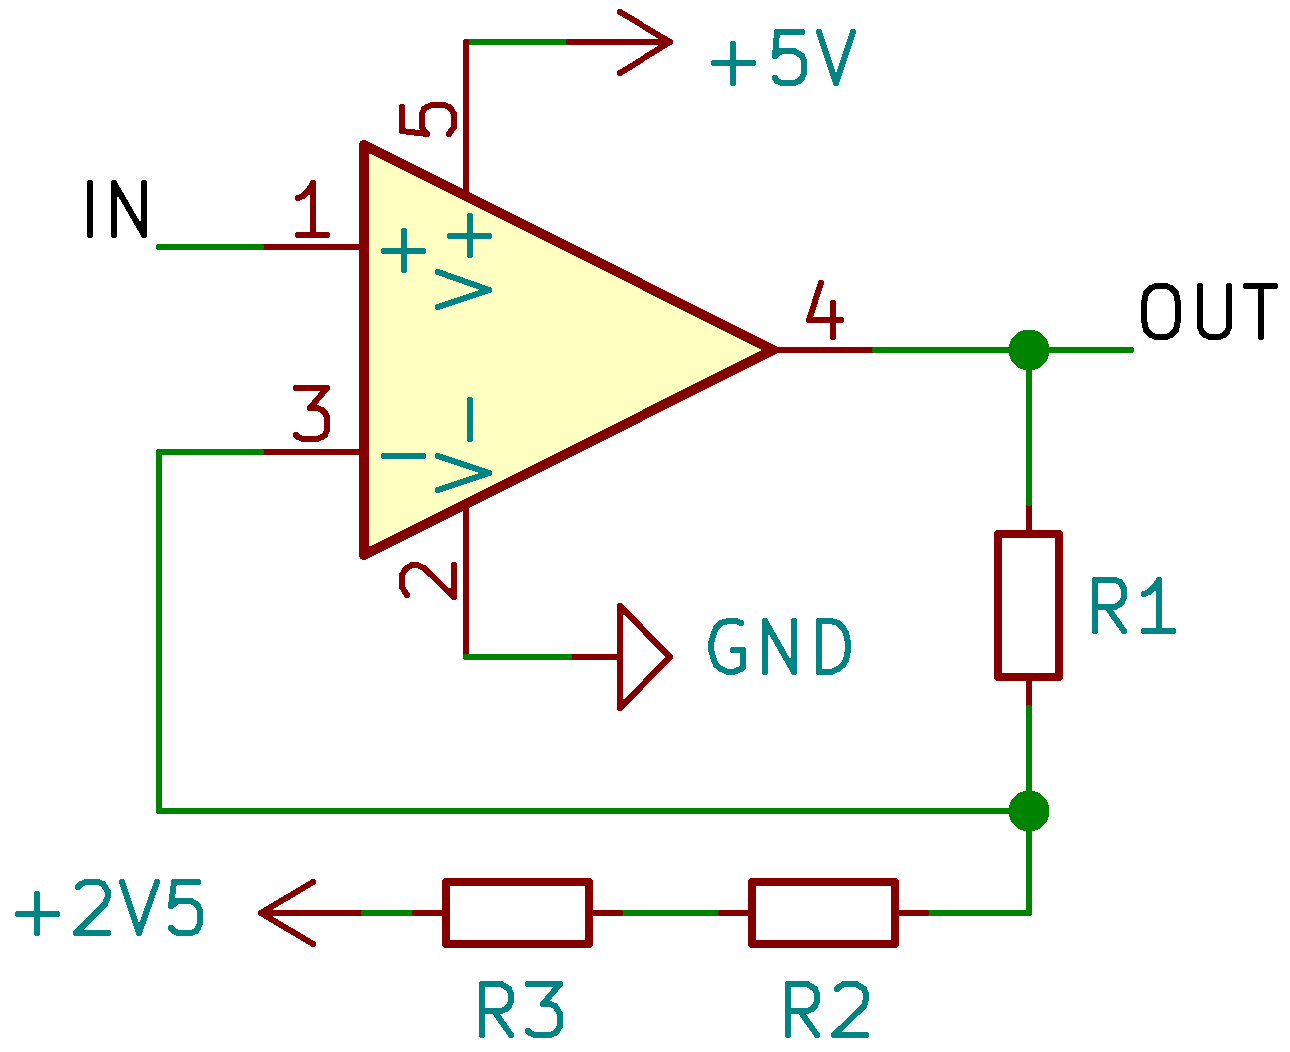
\includegraphics[width=0.3\textwidth]{gain_circuit}
	\caption{The non-inverting op-amp circuit.}
	\label{fig:non-inverting-op-amp}
\end{figure}

\begin{figure}[H]
	\centering
	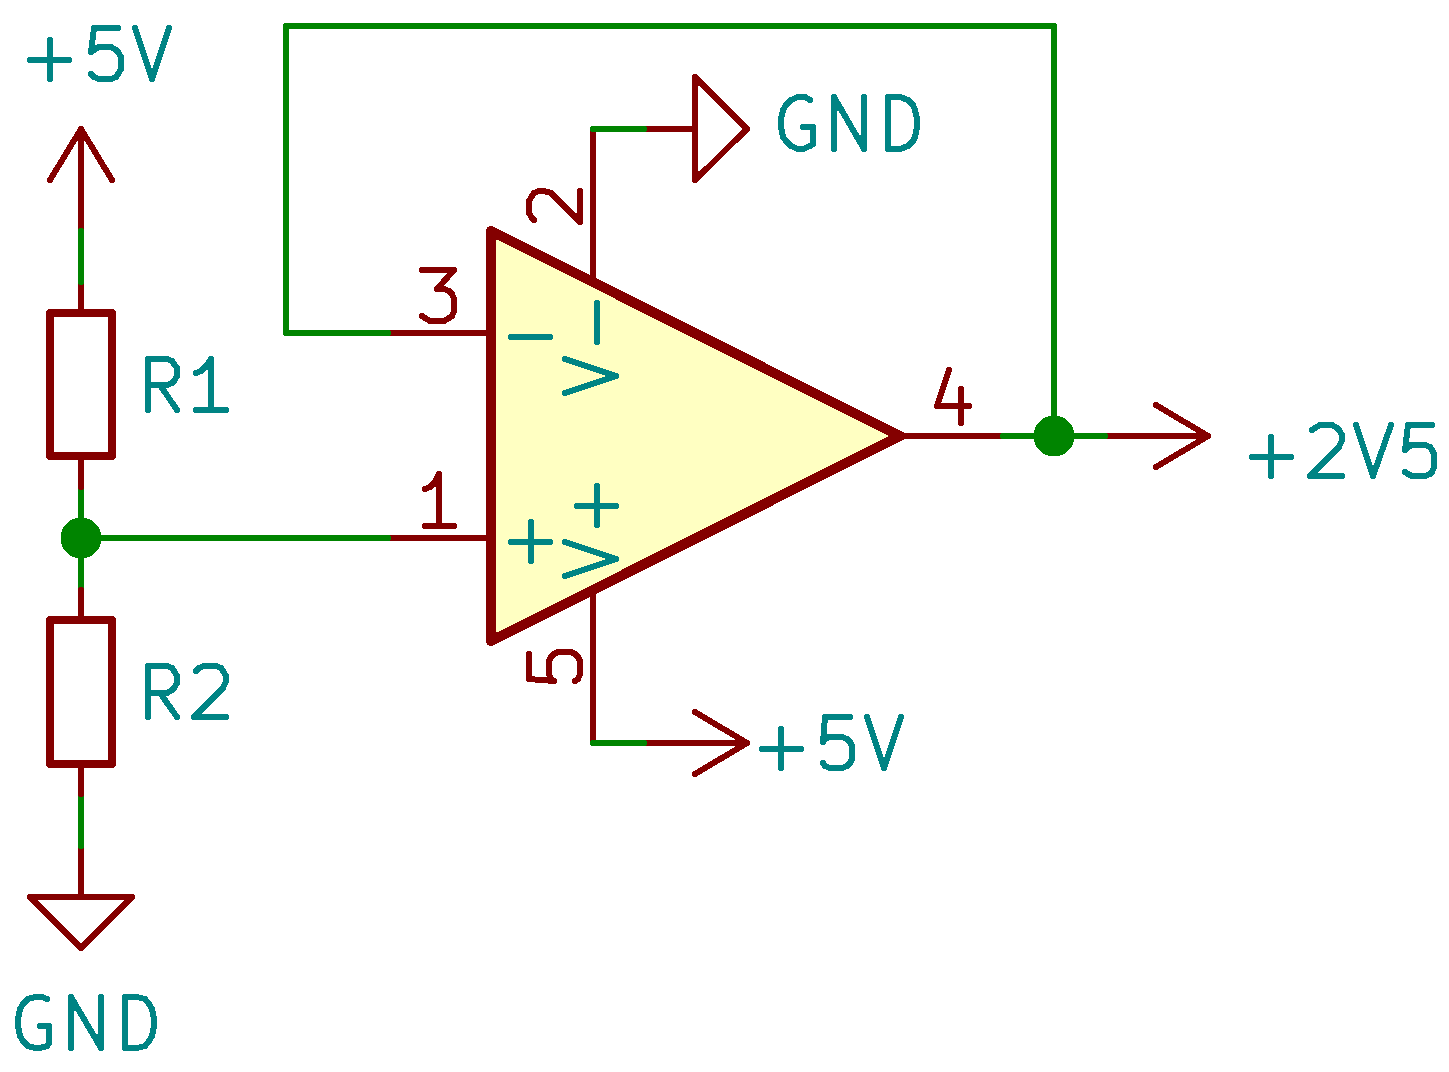
\includegraphics[width=0.3\textwidth]{virtual_ground_circuit}
	\caption{The virtual ground op-amp circuit.}
	\label{fig:half-supply}
\end{figure}

The op-amps are required to switch to a low power mode when no ADC readings are required.
Due to physical size constraints and part availability we have opted to disable the power supply to the op-amps to achieve a low power state.
The main drawback of this method is the start-up time to enable the op-amps.
The sum of the time taken to start the linear regulator and op-amp is less than $\SI{150}{\micro\second}$.

The source impedance is specified as being less than $\SI{100}{\ohm}$.
A higher input impedance is required for each op-amp circuit.
$Z_i = \SI{1}{\kilo\ohm}$ was decided upon, because it is 10 times higher than the worst-case source impedance.
Equations \ref{eq:r1} and \ref{eq:r2} show the derived formulae for the resistors based upon the given $Z_i$ and $A$ values.
\begin{align}
	R_1 &= Z_i A \label{eq:r1} \\
	R_2 + R_3 &= \frac{Z_i A}{A - 1} \label{eq:r2} \\[1em]
	\therefore R_1 = \SI{100}{\kilo\ohm}, R_2 &= \SI{1}{\kilo\ohm}, R_3 = \SI{10}{\ohm} \nonumber
\end{align}

The op-amps are required to switch to a low power mode when no ADC readings are taking place.
Due to physical size constraints and part availability we have opted to disable the power supply to the op-amps to achieve a low power state.
The main drawback of this method is the start-up time to enable the op-amps again.
The sum of the time taken to start the linear regulator and op-amp is less than $\SI{150}{\micro\second}$ (this is equivalent to $\SI{21.6}{\degree}$ of the $\SI{400}{\hertz}$ AC signal).

12 of these non-inverting amplifier circuits are required for each daughterboard.
The LMV324 selected as it has four op-amp circuits in one package, reducing the amount of space used on the board and the overall cost.
An additional package configured as unity gain amplifer produces the half-rail reference from a voltage divider input.
High value resistors are required in the divider (typically 100k$\omega$ to prevent excessive static current drain.
However these produce greater thermal noise, especially at high ambient temperatures, which is undesirable for ADC applications. Hence two 2k5$\omega$ balence nosie with 
static current drain of $\SI{1}{\milli\Amp}$

a 
Thermal calcuatins (not shown here for breitivy) show that the OpAmps will supply mimimal current into the microprocessor ADC inputs thus their power dissapation is reltively low.
Power dissabpatin is fiunction of the supply votage to ouput volateg diffence, ouput voalge diffenc to ground (for single suplkyt decies) and the ouput current.
With low power dissaption there is comfortable margin between the ambinent rempature of 105 degress, the gaurettened junction operting tempoate of 125 ddegress, and the device abolute maximu of 150 degrees.

Additnally worst case queincent current is 150uA.

\subsection{Microcontroller}




\subsection{Communications}















%%%%%%%%%%%%%%%%%%%%%%%%%%%%%%%%%%%%%%%%%%%%%%%%%%%%%%%%%%%%%%%%%%%%%%%%%%%%%%%%
%%%%%%%%                          EXAMPLE STUFF                         %%%%%%%%
%%%%%%%%%%%%%%%%%%%%%%%%%%%%%%%%%%%%%%%%%%%%%%%%%%%%%%%%%%%%%%%%%%%%%%%%%%%%%%%%

\newpage

\section{Example \LaTeX\ Stuff}

\LaTeX\ automatically typesets the text for you, so you don't need to worry about the formatting details for text.
If there is a blank line between two lines of text then they are considered different paragraphs, otherwise the paragraph is continued.

\textcolor{red}{Here is a line of red text.}
\textcolor{blue}{Here is a line of blue text.}

Referencing is done like this\cite{Varghese2012}. A bibliography is printed at the end of the report in IEEE style. A footnote can be added if required\footnote{Oh man, we should have started this last week!}.

\subsection{Math Mode}

Enter math mode by enclosing formulae in single dollar signs: $y(x) = e^x$.
To put the formula on its own line, use double dollar signs: $$c = \sqrt{a^2 + b^2}$$
To have multiple lines of math that are aligned properly on a symbol, then use the align environment:
\begin{align}
	\tan(\theta) &= \frac{\sin(\theta)}{\cos(\theta)} \\
		&= \frac{\sec(\theta)}{\csc(\theta)}
\end{align}
Note that a double back-slash makes a newline, the ampersand (\&) symbol sets the alignment.

If you don't want equation numbers, then put an asterisk (*) symbol after the environment name (this works for many things, like sections, etc):
\begin{align*}
	\tan(\theta) &= \frac{\sin(\theta)}{\cos(\theta)} \\
		&= \frac{\sec(\theta)}{\csc(\theta)}
\end{align*}

\subsection{Lists}

An example of the \texttt{enumerate} environment:
\begin{enumerate}
	\item One item.
	\item Another item.
	\item Yet another item.
\end{enumerate}

An example of the \texttt{itemize} environment:
\begin{itemize}
	\item One item.
	\item Another item.
	\item Yet another item.
\end{itemize}

\subsection{Images and Referencing}

Images can be included, such as figure \ref{fig:cat}. It may look a bit long-winded but using a figure environment allows you to give a caption and a label to the image. I usually just copy and paste figure blocks and change the caption, label and filename whenever I want another image. Labels are used to reference things somewhere else in the document (like this first sentence of this paragraph).

\begin{figure}[H]	% the capital H means that we'd like the image to appear exactly here in the document
					% if no letter is specified, LaTeX will put it where it thinks is best.
	\centering 		% centers the image on the page
	
\includegraphics[width=0.8\textwidth]{cat}	% this is where the image is inserted
												% we make the image 80% of the text width
												% the filename is `cat.jpg' and it lives in the images directory
												% LaTeX will find it without its filename extension
	\caption{Cat standing up.}	% the caption
	\label{fig:cat}	% give it a nice label. I like to use `fig' for figures, `eq' for equations, and `tab' for tables.
\end{figure}

Here's an example of referencing Pythagoras Theorem (equation \ref{eq:pythagoras}).
\begin{align} \label{eq:pythagoras}
	c^2 = a^2 + b^2
\end{align}




%%%%%%%%%%%%%%%%%%%%%%%%%%%%%%%%%%%%%%%%%%%%%%%%%%%%%%%%%%%%%%%%%%%%%%%%%%%%%%%%
%%%%%%%%                           BIBLIOGRAPHY                         %%%%%%%%
%%%%%%%%%%%%%%%%%%%%%%%%%%%%%%%%%%%%%%%%%%%%%%%%%%%%%%%%%%%%%%%%%%%%%%%%%%%%%%%%

\printbibliography

\end{document}
